\documentclass[10pt, a4paper,english,spanish,hidelinks]{article}
\usepackage{listings}
\usepackage{babel}
\usepackage{url}
\parindent = 0 pt
\parskip = 11 pt
\usepackage[width=15.5cm, left=3cm, top=2.5cm, height= 24.5cm]{geometry}

\usepackage{fancyhdr}
\usepackage{hyperref}
\usepackage{amsmath}
\usepackage{amsfonts}
\usepackage{amssymb}
\usepackage[utf8]{inputenc}
\usepackage{graphicx}
\usepackage{caption}
\usepackage{color}
\usepackage{subcaption}
\usepackage{appendix}
\usepackage{fancyhdr}
\usepackage{amsmath}

\pagestyle{fancy}
\lhead{Visión en Robótica}
\rhead{1er cuatrimestre 2013}

\setlength{\parindent}{0.8cm}
\setlength{\parskip}{\baselineskip}

\pretolerance=2000
\tolerance=3000

\begin{document}

\begin{titlepage}
\begin{flushright}
\textbf{\huge{Universidad de Buenos Aires}}\\
\vspace*{10pt}
\textbf{\LARGE{Facultad de Ciencias Exactas y Naturales}}\\
\vspace*{10pt}
\textbf{\Large{Departamento de Computación}}\\
\vspace*{10pt}
\textbf{\Large{Visión en Robótica}}\\
\end{flushright}

\vspace*{5cm}

\begin{center}
 \Huge{\textbf{Proyecto Final \\ \textit{}}}
\end{center}
\vspace*{7cm}
\Large{
\begin{flushright}
Lambrisca, Santiago - 274/10 - santiagolambrisca@gmail.com\\
Rebecchi, Alejandro - 15/10 - alejandro.rebecchi@outlook.com\\
Gauder, María Lara - 27/10 - marialaraa@gmail.com\\
\end{flushright}
}
\end{titlepage}


\lstset{language=c, breaklines=true, basicstyle=\footnotesize}
\lstset{numbers=left, numberstyle=\tiny, stepnumber=1, numbersep=-2pt}


\newpage
\section{Introducción}
El objetivo de este trabajo práctico final es el de poder obtener el camino
realizado por un robot un otro objeto a partir de un video capturado por una cámara a bordo.
Comparando las imágenes capturadas se podrá obtener la matriz de rotación y traslación realizada 
por el mismo en ese tiempo. A partir de esas matrices se obtienen las posiciones por las que
el robot ha pasado. Se establece la posición del objeto al comienzo del video como el punto inicial,
cuyas coordenadas $x$ e $y$ tendrán como valor cero. 

\section{Desarrollo}
Para reconstruir el camino lo hacemos de forma constructiva comparando cuadros del video (o ``frames'') de a dos y calculando la 
rotación y traslación necesaria para pasar de la cámara del primer ``frame'' a la del otro. De esta forma obtenemos para cada para de
cuadros la posición relativa en uno con respecto al otro, por lo que haciéndolo de forma consecutiva podemos reconstruir la
totalidad del recorrido. Éstas transformaciónes las obtenemos a partir de la matriz escencial, la cual también calculamos para
cada par de frames que procesamos.

Como disponemos de una función para calcular la matriz fundamental para dos frames, podremos obtener la matriz
esencial valiéndonos de la fórmula
\begin{equation}
E = K^t * F * K
\end{equation}
donde $E$ es la matriz escencial, $F$ la fundamental y $K$ la de calibración de la cámara. Calculamos la matriz fundamental de forma directa 
y a partir de ella obtenemos la matriz escencial. 

La matriz de calibración de las cámaras se encuentra calculada previamente. Dado que siempre es la misma 
cámara la que se utiliza para tomar las imágenes dichos valores se mantienen constantes.

La matriz fundamental se obtiene a partir de una función brindada 
por las librerías OpenCV. La misma requiere únicamente de los puntos de correspondencia entre las dos 
imágenes a comparar los cuales son obtenidos mediante la función
\textit{get\_correspondence} previamente y almacenados luego en dos vectores (uno contiene
los puntos de una imagen y el otro de la otra).

Una vez obtenida la matriz escencial, lo siguiente es calcular las matriz de las cámaras  
$P$ y $P'$ que corresponden al primer y segundo frame respectivamente. Si asumimos que \textit{P}
es la cámara canónica,
\begin{equation}
P  = K[ I | 0 ]
\end{equation}
\begin{equation}
P' = K[ R | T ]
\end{equation}
solo es necesario calcular $P'$ para obtener la matriz de rotación y traslación 
entre dichas matrices de las cámara. 

La matriz perteneciente a la cámara $P'$ en principio, presenta cuatro opciones diferentes, dado
que se compone de dos posibles traslaciones y otras dos rotaciones. Las mismas se
presentan a continuación:
\begin{equation}
 R_{1} = U * W^t * V^t
\end{equation}
\begin{equation}
 R_{2} = U * W * V^t 
 \end{equation}
\begin{equation}
 T_{1} = T 
 \end{equation}
\begin{equation}
 T_{2} = -T
\end{equation}
donde 
\[ W = \left( \begin{array}{ccc}
0 & -1 & 0 \\
1 & 0 & 0\\
0 & 0 & 1\end{array} \right).\] 
y las matrices U y V son obtenidas de la descomposión SVD de \textit{E} a partir de la función 
\textit{compute}. En caso de que el $det(V^{t})$ o el $det(U)$ sean menores a cero, se calcula
la descomposión a partir de la matriz \textit{-E}.

Por otro lado la matriz $T$ se obtuvo mediante la descomposión $E * T = 0$ recurriendo
a la función \textit{solveZ} de la librería SVD. 

Una vez determinadas las cuatro posibles $P'$, se deberá decidir cuál es la correcta,
es decir en la que los puntos de la imagen queden delante del plano. Para ello
se obtendrán las posiciones $Q$ en el mundo para todos los puntos asociados a las correspondencias (en el homogéneo). 
La obtención de las posiciónes se realiza mediante la función \textit{triangulatePoints}
que define de manera automática la $Q$ adecuada para un par de puntos de la 
correspondencia del par de imágenes y una posible
matriz de la cámara $P'$. Dicho punto deberá cumplir que 
\begin{equation}
 Q_z * Q_w > 0 \land (P'Q)_z * Q_w > 0 \leftarrow
\end{equation}
Dado que ésto se calcula para todos los puntos, se quiere tomar como la matriz correcta la que cumpla 
dicha condición para la mayor cantidad de correspondencias. Por lo tanto  se tiene un contador para cada una de las
cuatro opciones de $P'$ y se incrementa el correspondiente a la matriz que se toma como correcta para cada correspondencia.
En caso de que no haya ninguna válida no se suma a ningun contador. Esto se debe a que ese par de puntos es considerado un outlayer.
Por último, se extrae de la matriz de la cámara $P'$, correspondiente al contador de mayor valor, las matrices de rotación y traslación. 


Para poder obtener la posicion en la que se encuentra el objeto luego de cierta cantidad
de ``frames'', se debe calcular la rotación y traslación con respecto al eje de coordenadas original.
Para esto se deberá acumular las rotaciones en una matriz que sea el producto de todas las rotaciones previas.
Luego dicha matriz deberá multiplicarse por la matriz de traslación y sumar ésto a la última posición del objeto obtenida hasta el momento para obtener la actual.
Para poder mejorar la precisión en los cálculos, se decidió normalizar la matriz de rotación
y a la matriz de traslación se la divide por la tercera componente. 

\newpage
\section{Resultados}
Una vez finalizado el desarrollo del algoritmo, se aplicó el mismo a dos videos 
brindados por la cátedra. En primer lugar se podrá observar el camino realizado por el
robot a partir de la coordenada $x$ e $y$. Se utilizó para poder graficar los puntos
obtenidos el programa octave, que
guarda una imagen con el gráfico obtenido. 

\centerline{ }
\centerline{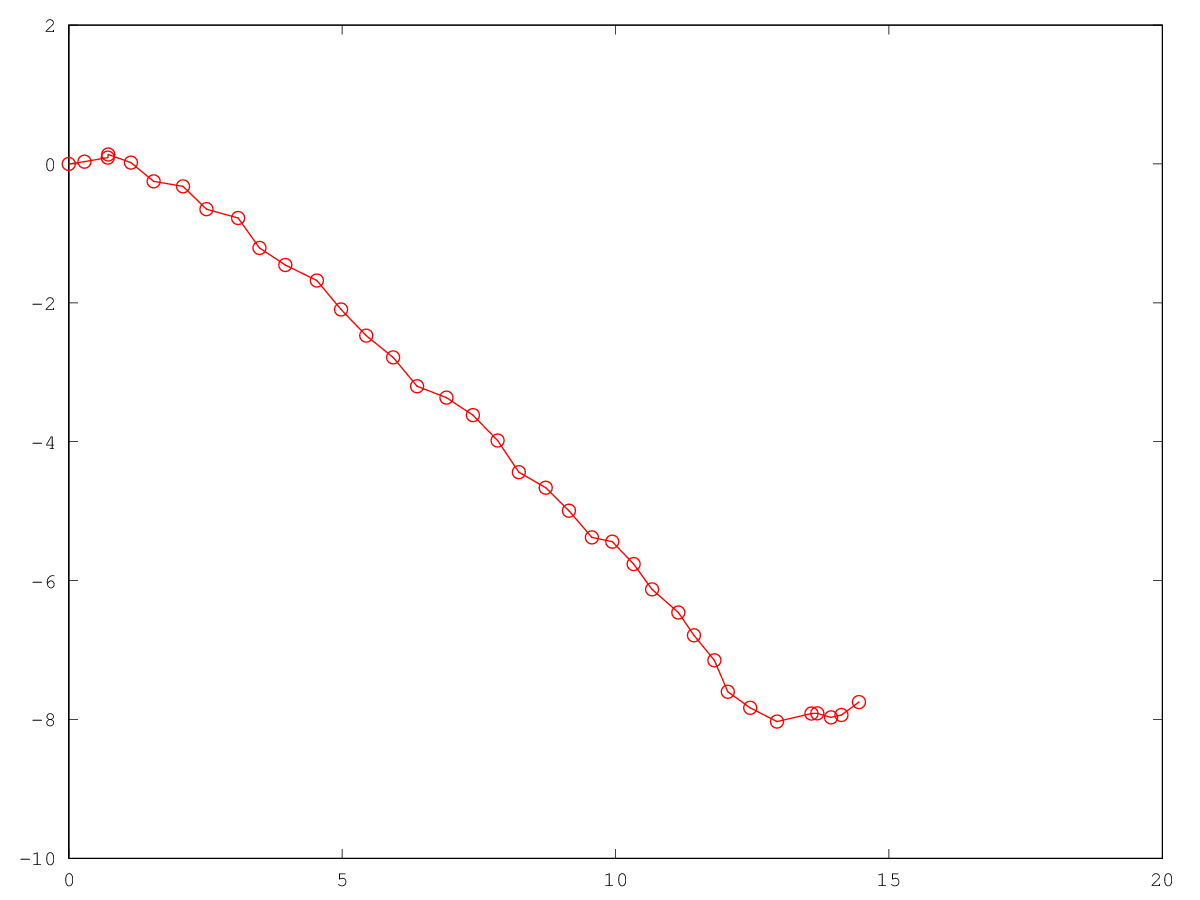
\includegraphics[width=0.7\textwidth]{./img/recto1.png}}
\centerline{\textbf{Video}: recto1; con 20 cuadros de diferencia.} 

\centerline{ }
\centerline{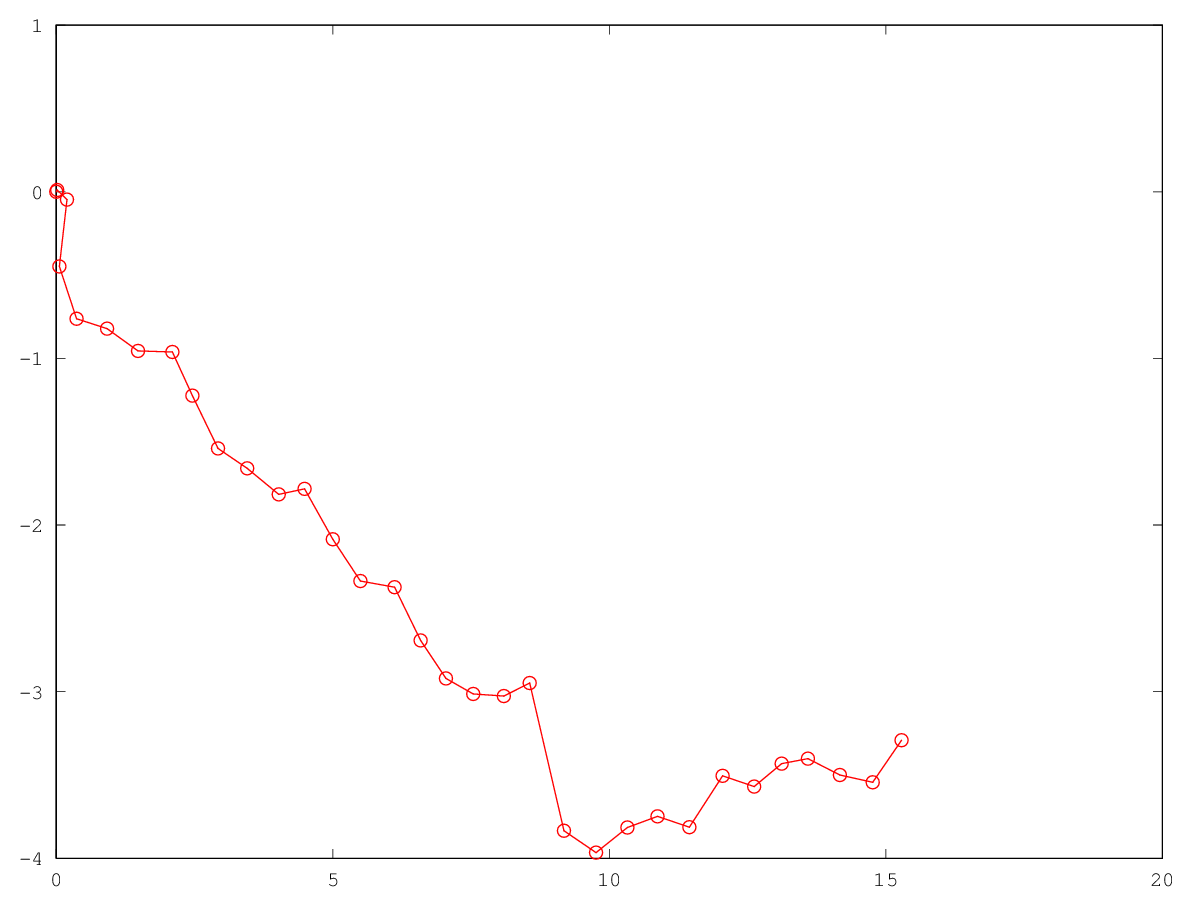
\includegraphics[width=0.7\textwidth]{./img/recto2.png}}
\centerline{\textbf{Video}: recto2; con 20 cuadros de diferencia.} 

\centerline{ }
\centerline{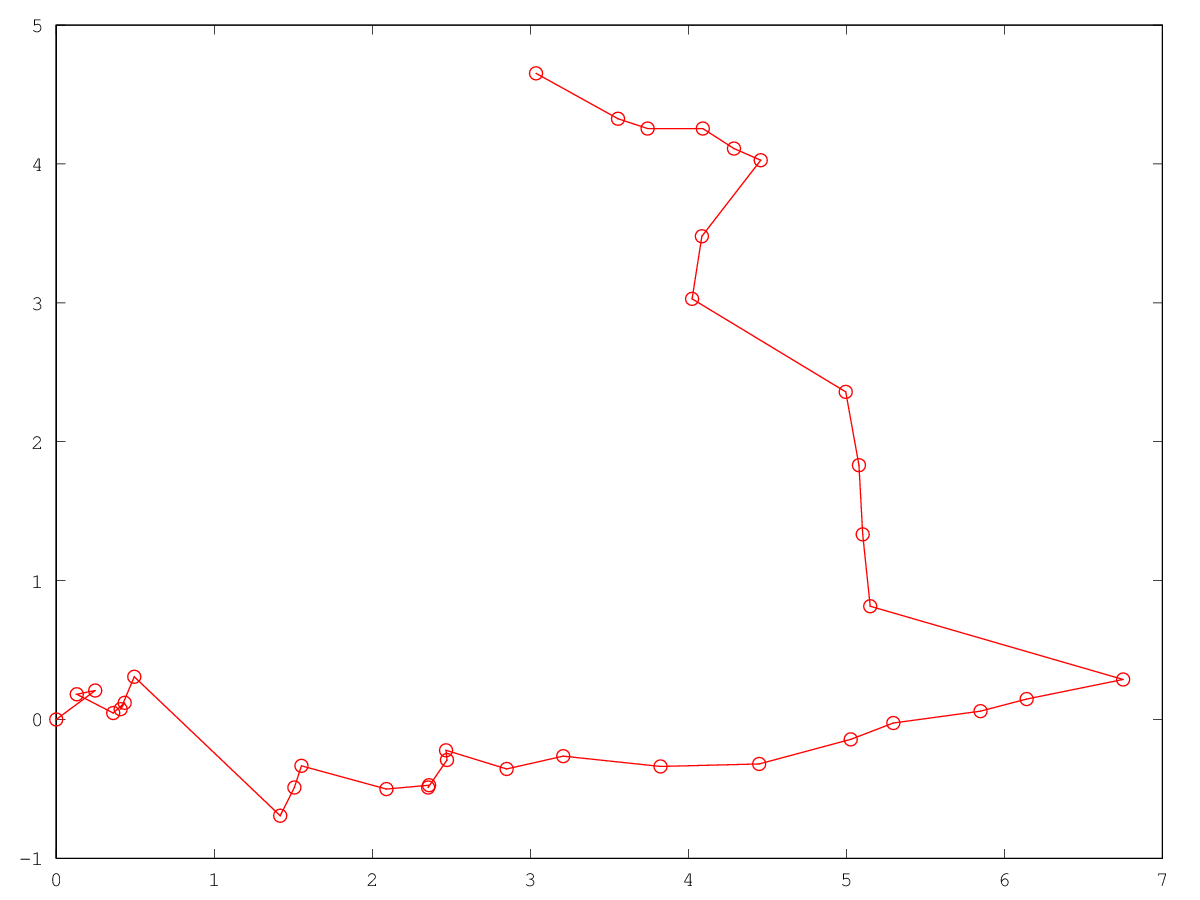
\includegraphics[width=0.7\textwidth]{./img/recto3.png}}
\centerline{\textbf{Video}: recto3; con 40 cuadros de diferencia.}

En ambas imágenes se observa una similitud de acuerdo a los movimientos realizado por
el robot en su trayectoria. A continuación se muestran experimentaciones realizadas con
esos mismos videos pero modificando la cantidad de ``frames'' que se ignoran en la comparación
de las imágenes. 

\centerline{ }
\centerline{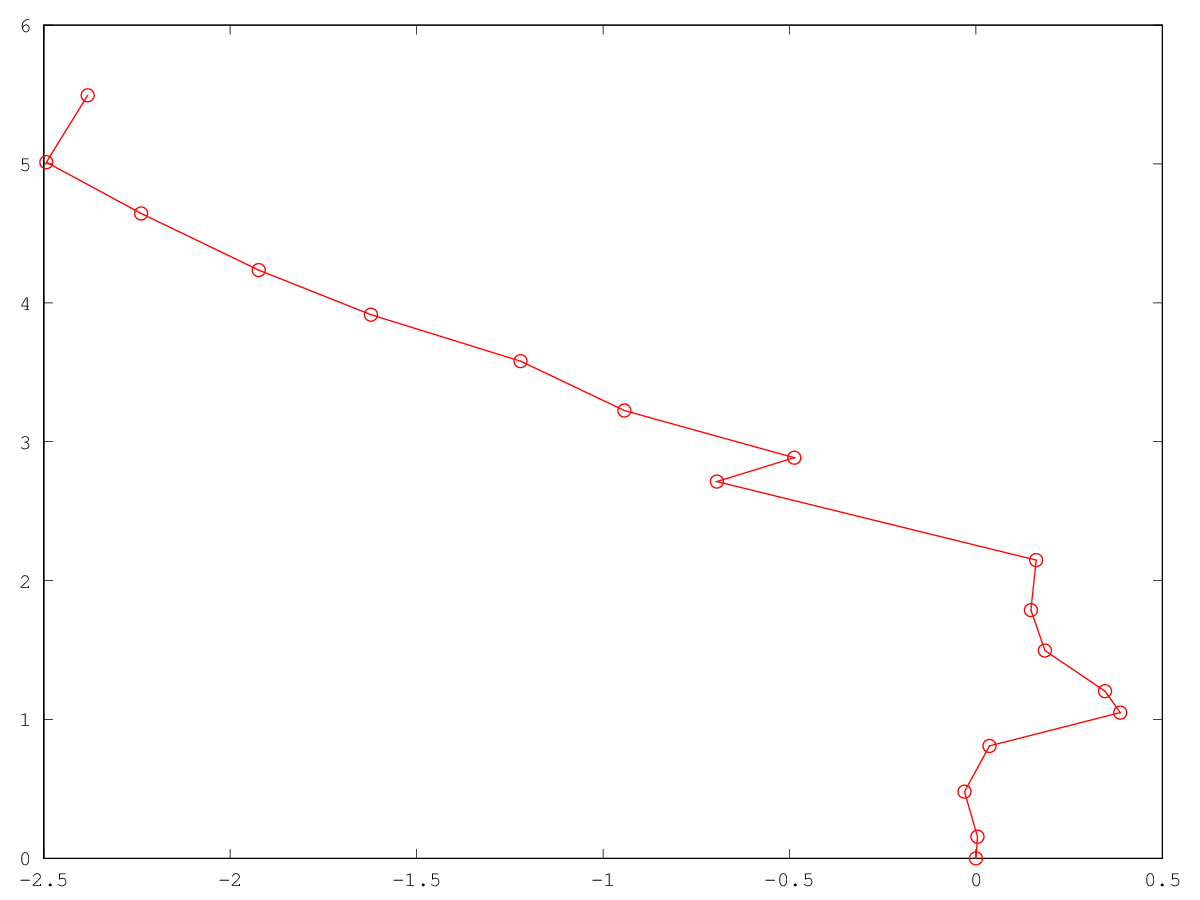
\includegraphics[width=0.7\textwidth]{./img/r2cant40.png}}
\centerline{\textbf{Video}: recto2; con 40 cuadros de diferencia.} 

Lo cual se puede notar que no se distinguen bien los pasos realizados por el objeto, ya
que en los cuadros desperdiciados se realizaban varios movimientos. 
Por último, queremos mostrar que ocurre en el caso de que el movimiento tambien implica una rotación.
%\centerline{ }
%\centerline{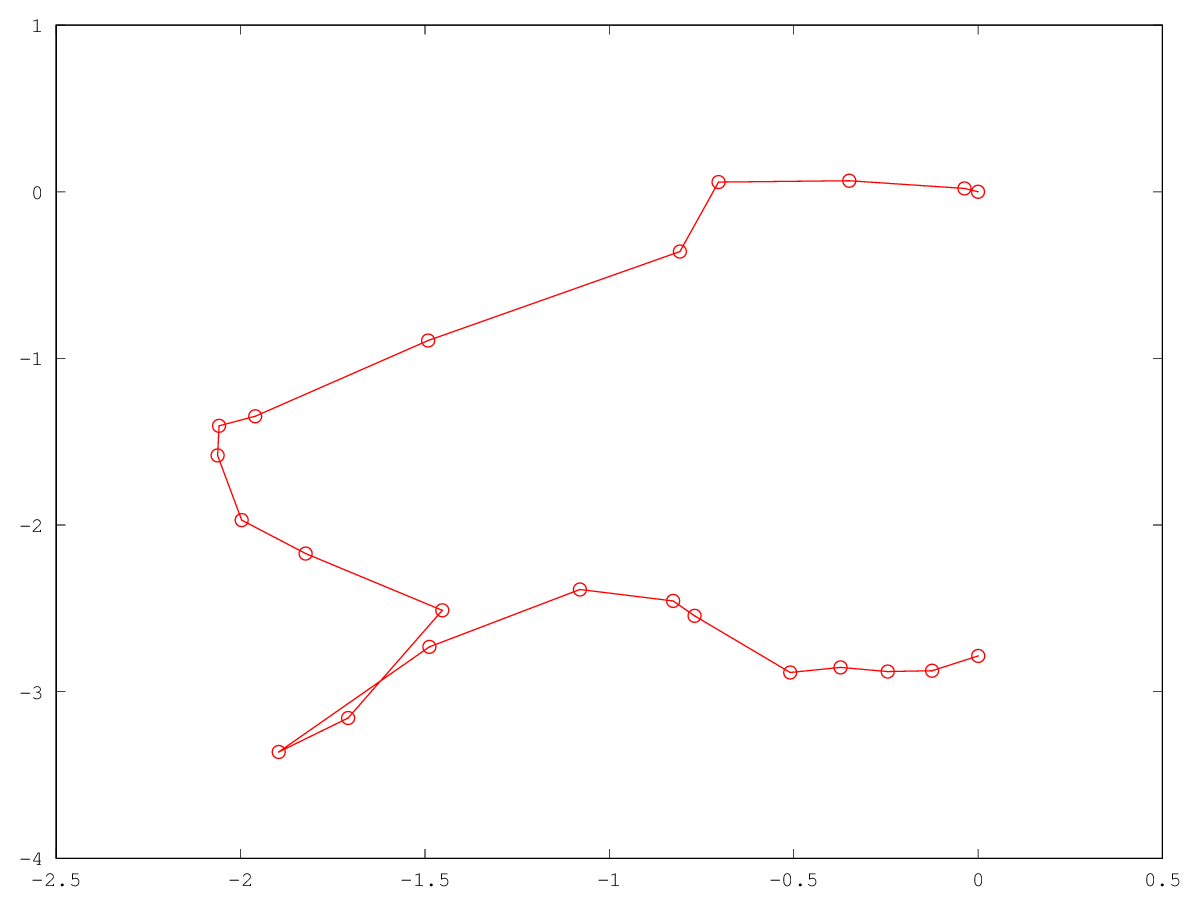
\includegraphics[width=0.7\textwidth]{./img/rotacion40.png}}
%\centerline{Video: rotacion; con 40 cuadros de diferencia.}
%\centerline{ }
%\centerline{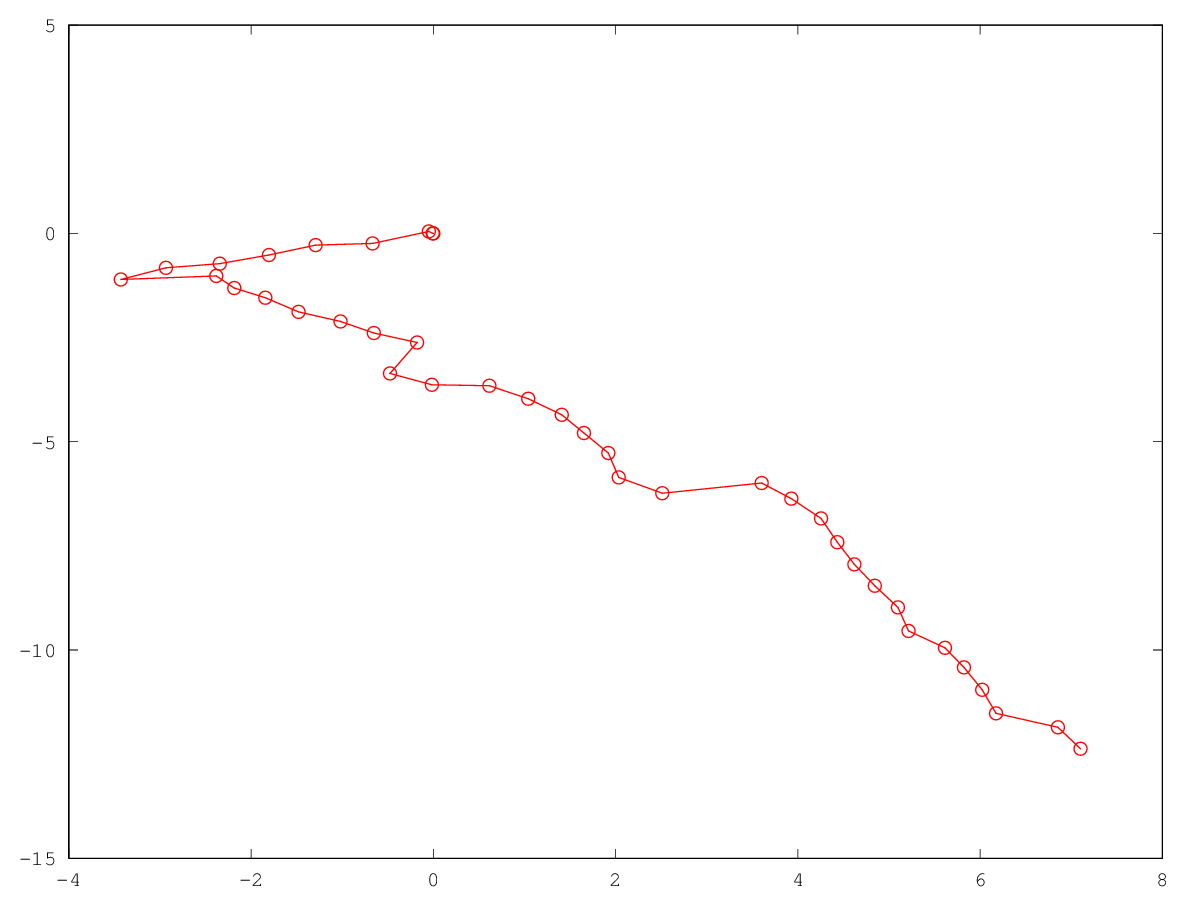
\includegraphics[width=0.7\textwidth]{./img/semi-circulo1-20.png}}
%\centerline{Video: semi-circulo1; con 20 cuadros de diferencia.}
%\centerline{ }
%\centerline{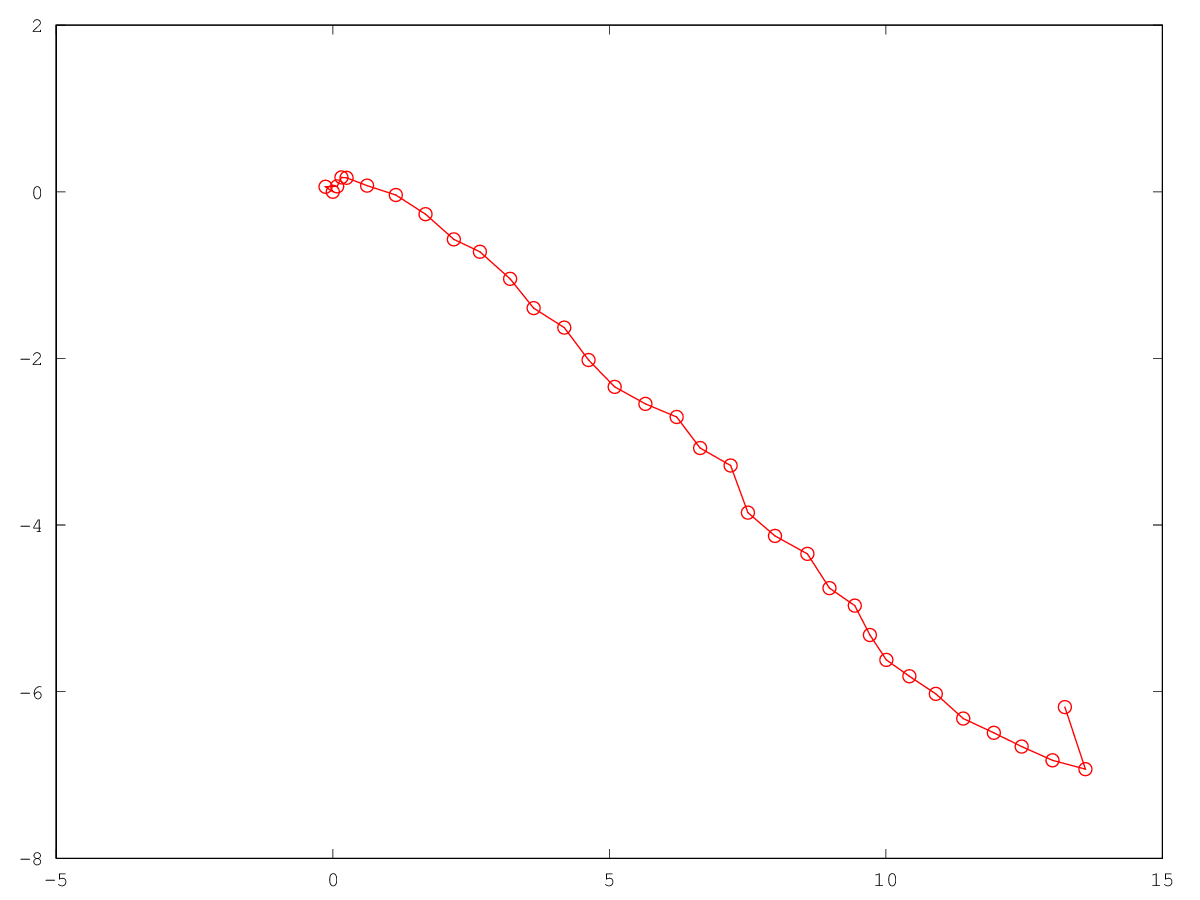
\includegraphics[width=0.7\textwidth]{./img/semi-circulo2-27.png}}
%\centerline{Video: semi-circulo2; con 27 cuadros de diferencia.}
%\centerline{ }
%\centerline{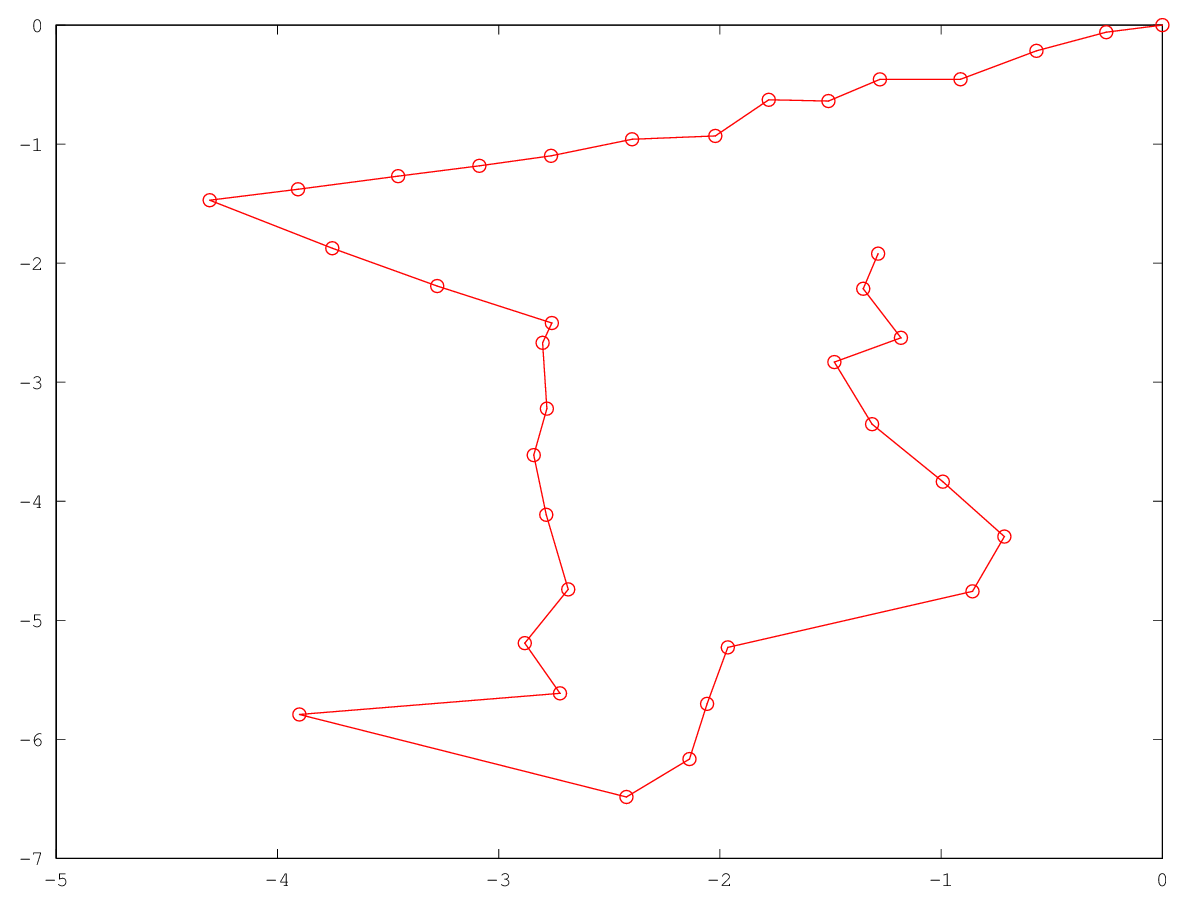
\includegraphics[width=0.7\textwidth]{./img/semi-circulo3-20.png}}
%\centerline{Video: semi-circulo3; con 20 cuadros de diferencia.}
%\centerline{ }
%\centerline{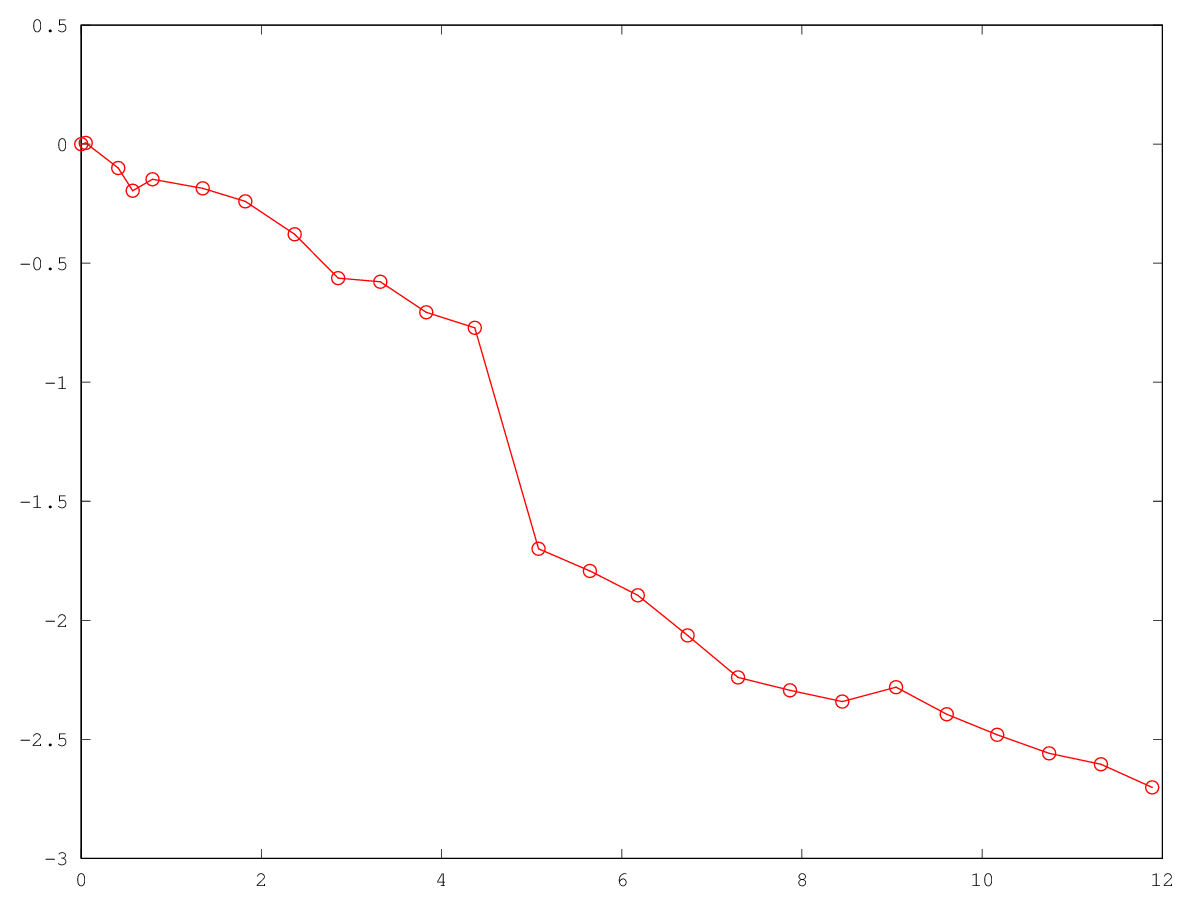
\includegraphics[width=0.7\textwidth]{./img/zigzag-40.png}}
%\centerline{Video: zigzag; con 40 cuadros de diferencia.}

\begin{center}
\begin{tabular}{c c} 
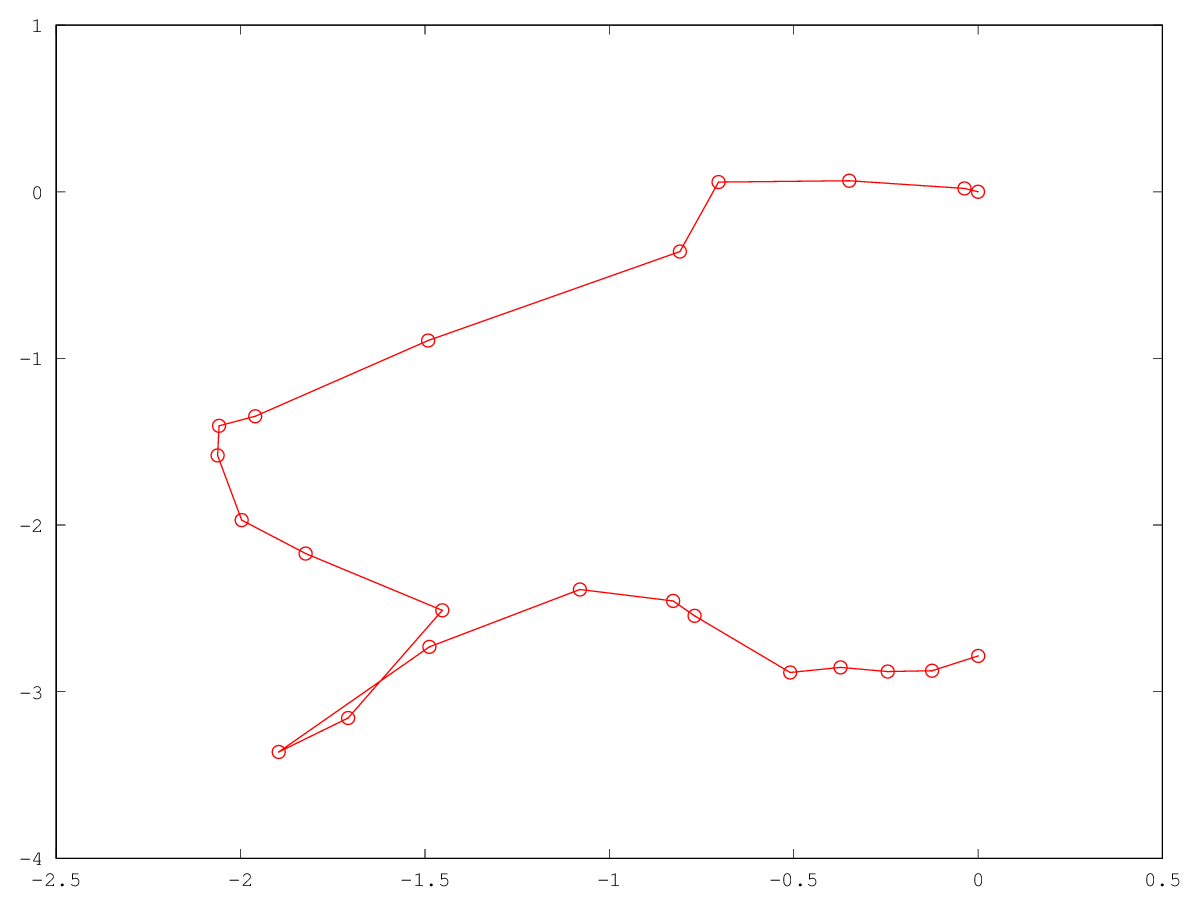
\includegraphics[width=0.5\textwidth]{./img/rotacion40.png} &
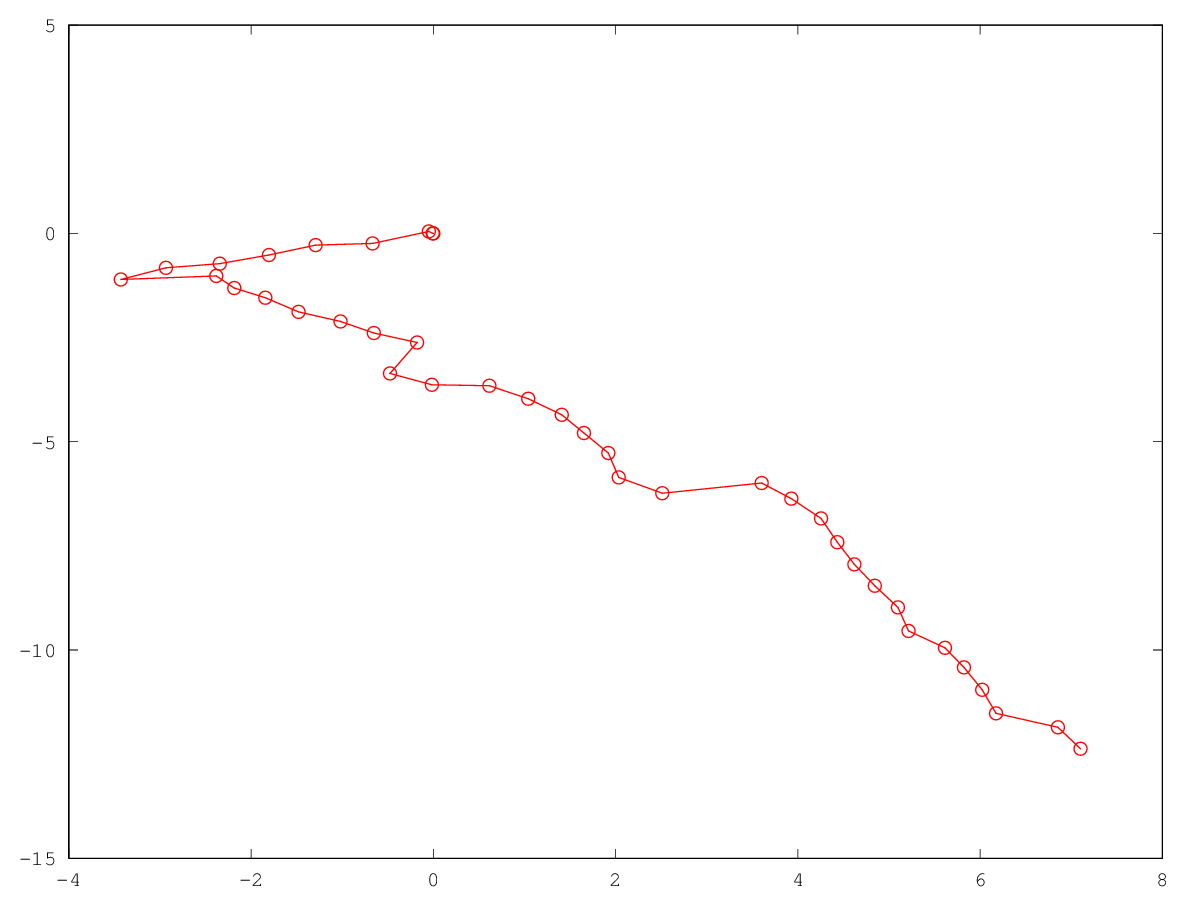
\includegraphics[width=0.5\textwidth]{./img/semi-circulo1-20.png} \\
 \small{\textbf{Video}: rotacion; con 40 cuadros de diferencia.} &
 \small{\textbf{Video}: semi-circulo1; con 20 cuadros de diferencia.} \\
 \end{tabular}
\end{center}
\begin{center}
\begin{tabular}{c c} 
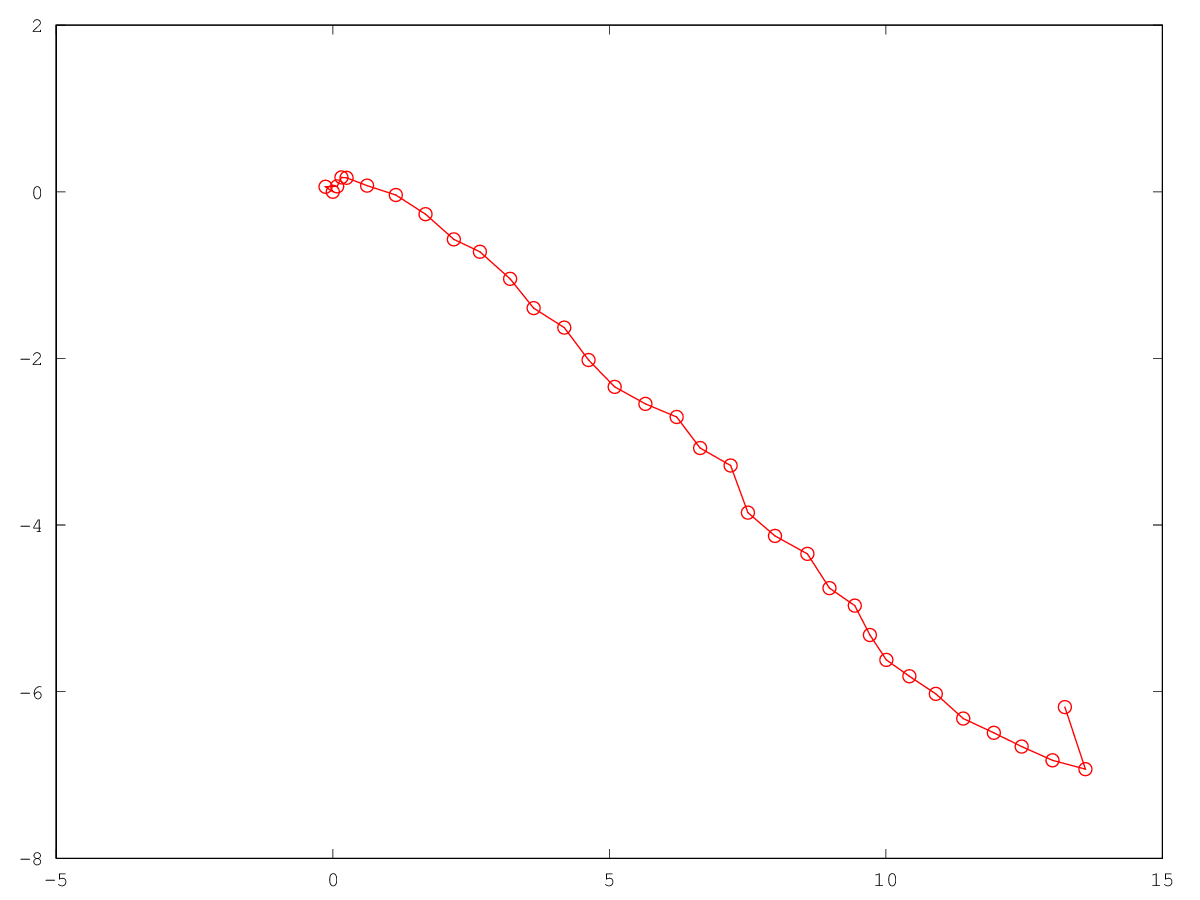
\includegraphics[width=0.5\textwidth]{./img/semi-circulo2-27.png} &
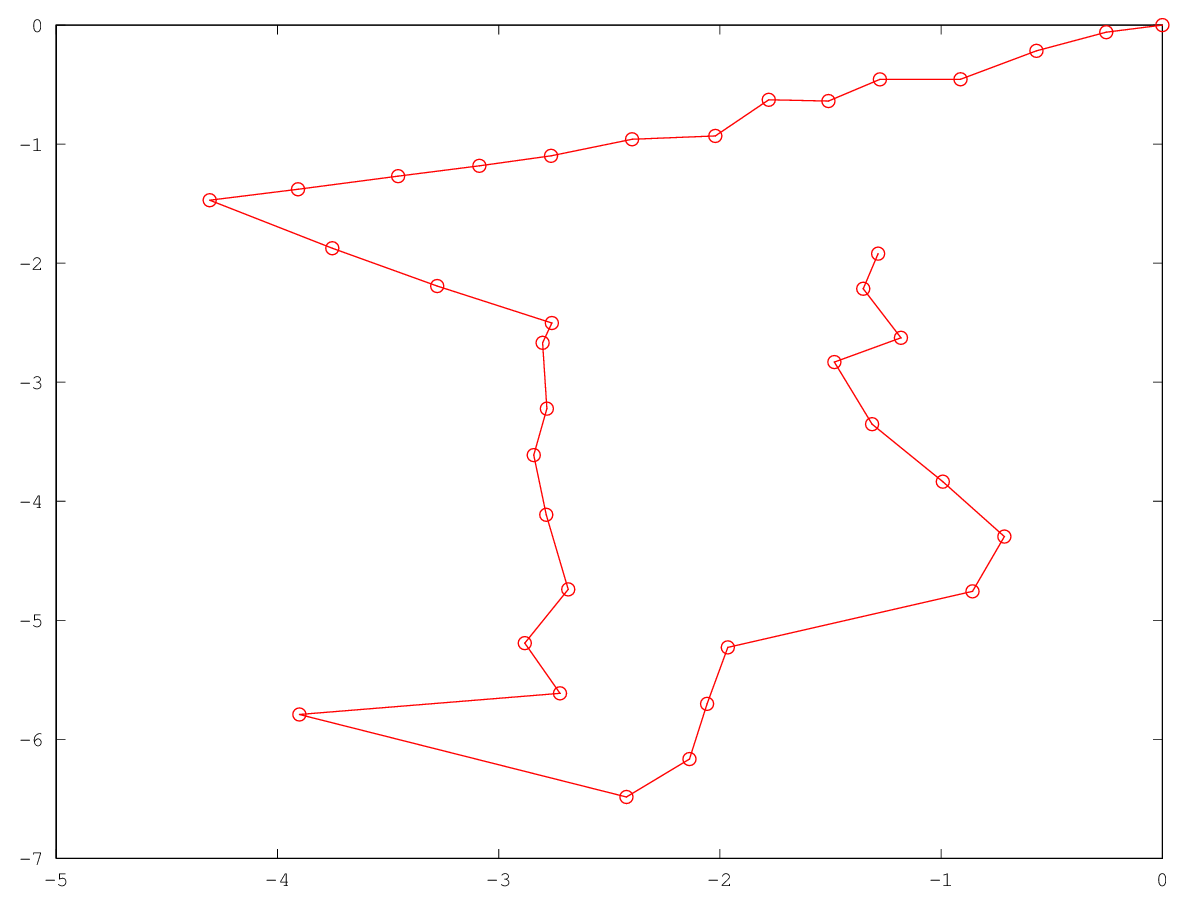
\includegraphics[width=0.5\textwidth]{./img/semi-circulo3-20.png} \\
 \small{\textbf{Video}: semi-circulo2; con 27 cuadros de diferencia.} &
 \small{\textbf{Video}: semi-circulo3; con 20 cuadros de diferencia.} \\
 \end{tabular}
\end{center}
\centerline{ }
\centerline{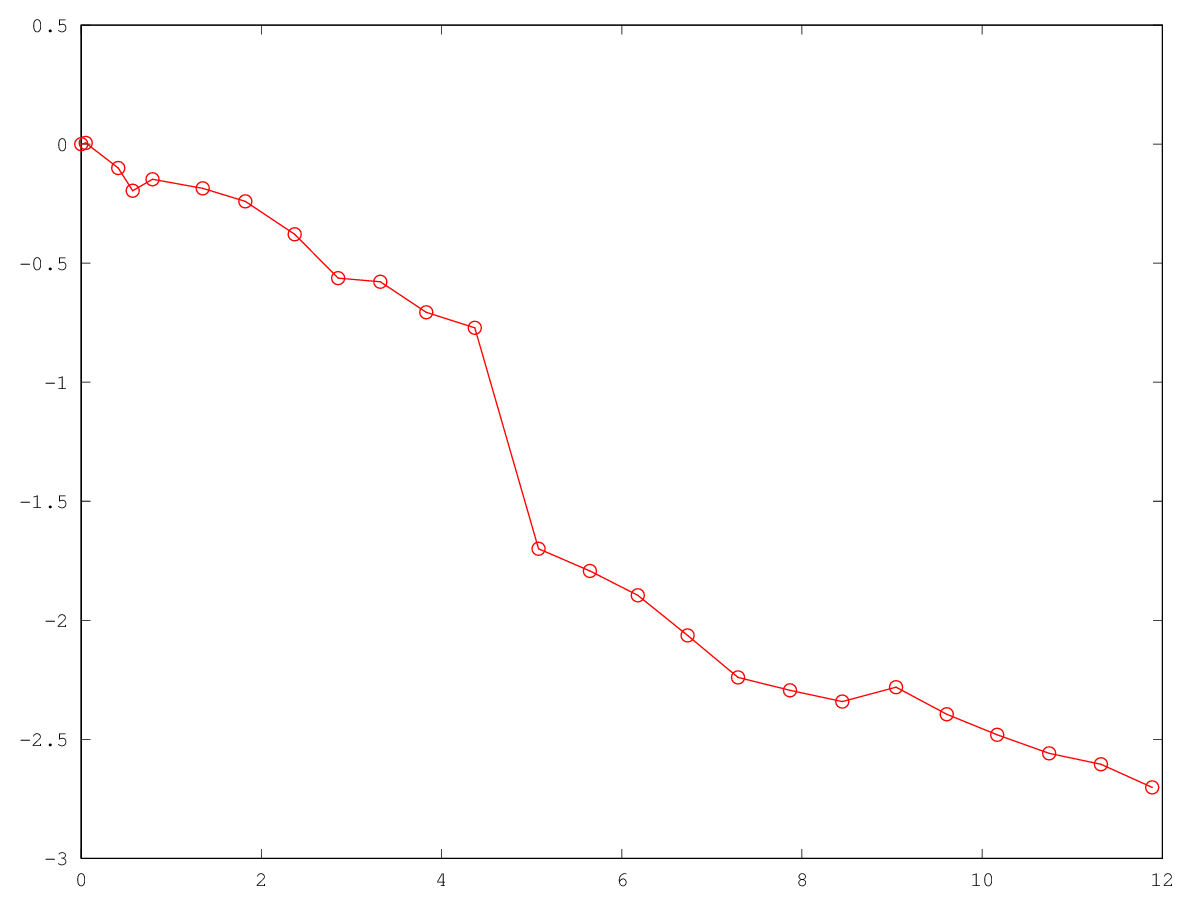
\includegraphics[width=0.6\textwidth]{./img/zigzag-40.png}}
\centerline{\textbf{Video}: zigzag; con 40 cuadros de diferencia.}

Los gráficos obtenidos muestran que la estimación de las trayectorias para este tipo de movimientos, no se aproxima a la real.
Esto se debe a que al acumularse las rotaciónes también lo hacen los errores en el calculo de ellas, y este es mas sensible al tener una rotación mayor.

\end{document}
